\chapter{Condensate Fraction}\label{CondFrac}

Consider the Bose-Hubbard Hamiltonian
\begin{equation}
	\hat{H} = -J \sum_{\braket{i,j}} \hat{a}_{i}^{\dag} \hat{a}_j + \frac{U}{2} \sum_{i} \hat{n}_i \left( \hat{n}_i -1 \right) \; , 
\end{equation}
which describes nearest-neighbour interactions in a one-dimensional lattice. This Hamiltonian supports two distinct quantum phases: The Superfluid (SF) phase, $U/J \ll 1$, which exhibit long range correlations, and the Mott-Insulator (MI) phase, $U/J \gg 1$, where sites are isolated, hence no correlation between sites is present. The SF phase is a Bose-Einstein condensate with special attributes, as it exhibits maximal de-localization of the particles and can be approximated as a coherent state. On the other hand, as the individual sites are completely decoupled in the MI phase, no condensate is present. \\
According to the Penrose-Onsager criterion, a Bose-Einstein condensate, and by extension the SF state, is present if and only if the largest eigenvalue, $\lambda_1$, of the single-particle density matrix, $\rho^{(1)}$, is macroscopic
\begin{equation}
	f_c = \frac{\lambda_1}{N_{\mathrm{particles}}} > 0 \; ,
\end{equation} 
where $f_c$ is the \textit{condensate fraction} and $N_{\mathrm{particles}}$ is the total number of particles. Thus, the condensate fraction can be used to determine which state is the dominant of the system, as
\begin{align}
	\lim_{N_{\mathrm{particles}} \to \infty} f_{c}^{\mathrm{SF}} &\to 1 \label{eq:SF_lim} \\
	\lim_{N_{\mathrm{particles}} \to \infty} f_{c}^{\mathrm{MI}} &\to 0 \; , \label{eq:MI_lim}
\end{align}
where the filling-fraction $n = N_{\mathrm{particles}}/N_{\mathrm{sites}}$ is held constant. While the limit for the SF phase will be reached for any number of particles, the MI phase will only be reached in the limit $N_{\mathrm{particles}} \to \infty$.

\section{Numerical Results}
In order to test the precision of MPS formalism and the ITensor library, the condensate fraction was calculated for a series of $U/J$ with varying particle number. For this the library's DMRG algorithm was used, where the number of sweeps was selected such that the bond dimension remained the same when adding more sweeps. In this case 5 sweeps with a maximum bond dimension of 200 was sufficient. All calculations were performed with unit occupancy. These results were then compared to a similar calculation using exact diagonalisation.

\begin{figure}[h!]
    \centering
    \begin{subfigure}[t]{0.49\textwidth}
        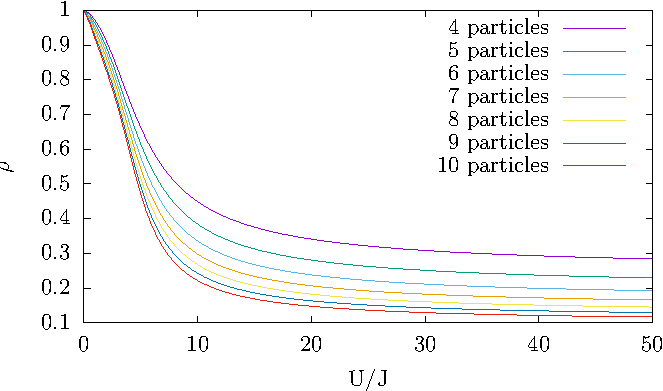
\includegraphics[width=\textwidth]{Figures/Condfrac_4to10.pdf}
        \caption{\textit{Condensate fraction calculated from an MPS after performing 5 DMRG sweeps.}}
        \label{fig:Condfrac_4to10}
    \end{subfigure}
    ~
    \begin{subfigure}[t]{0.49\textwidth}
        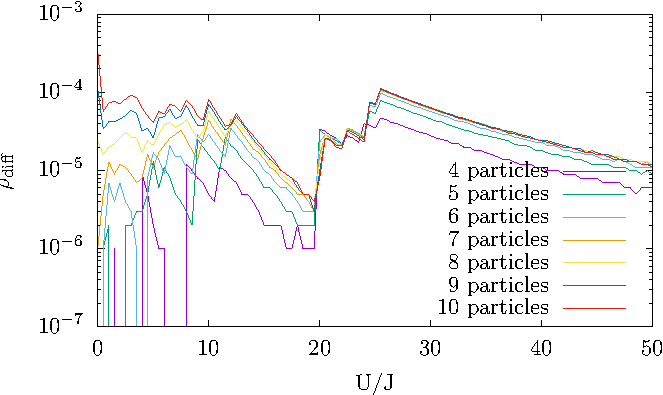
\includegraphics[width=\textwidth]{Figures/Confrac_exactvsMPS.pdf}
        \caption{\textit{Absolute difference between the condensate fraction calculated using MPS and using exact diagonalisation.}}
        \label{fig:Condfrac_exactvsMPS}
    \end{subfigure}    
\end{figure}
Figure \ref{fig:Condfrac_4to10} shows the condensate fraction for various $U/J$ calculated using MPS. In the limit $U/J = 0$ the condensate fraction is 1 as expected, thus confirming that the system is in the SF state. Meanwhile, in the limit $U/J = 50$ the condensate fraction is dependent on the number of particles, however, this is just as equation \ref{eq:MI_lim} describes.\\
In figure \ref{fig:Condfrac_exactvsMPS} the results of the MPS calculation is compared to exact diagonalisation by displaying the absolute difference between the two calculations. It is clear that the two approaches yield very similar results for low particle-number.\\
One of the great advantages of MPS is its ability to accurately describe states with a large number of particles, which is unfeasible with exact diagonalisation. 
\begin{figure}[h!]
	\centering
	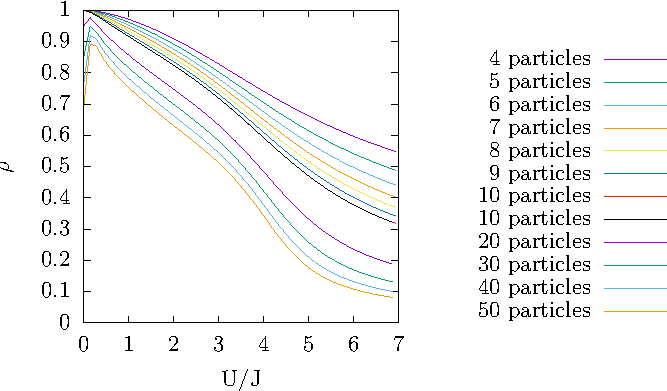
\includegraphics[width=0.9\textwidth]{Figures/Condfrac_4to50.pdf}
	\caption{\textit{Condensate fraction calculated from an MPS after performing 20 DMRG sweeps.}}
	\label{fig:Condfrac_4to50}
\end{figure}
Figure \ref{fig:Condfrac_4to50} shows the results of the DMRG calculations for up to 50 particles. The condensate fraction behaves as expected in the $U/J \gg 1$ limit, as it tends towards zero for larger particle numbers. Note, however, that in the SF limit the results are not quite as expected, as the condensate fraction does not reach 1. This is a consequence due to the way MPS' are constructed, which makes it very hard to accurately describe the very long ranged correlations of the Superfluid.


\subsection{Correlations in Matrix Product States}
In order to understand why MPS struggles with describing the SF correlations, one can take advantage of the \textit{transfer operator}.
Consider an MPS of the form
\begin{equation}
	\ket{\psi} = \sum_{\{ j \} } \left( \prod_{n \in \mathbb{Z}} M^{j_n} \right) \ket{\{ j \}} \; ,
\end{equation}
where the $M$'s are the matrices of the MPS, and $j_n$ are the physical indices. The transfer operator is defined as
\begin{equation}
	\hat{E}^{[n]} = \sum_{\alpha_{n-1}, \alpha_{n-1}'} \sum_{\alpha_{n}, \alpha_{n}'} \left( \sum_{j_n} M^{[n] j_n *} \otimes  M^{[n] j_n} \right)_{(\alpha_{n-1} \alpha_{n-1}'),(\alpha_{n}  \alpha_{n}')} \left( \ket{\alpha_{n-1}}\bra{\alpha_{n-1}'} \right) \left( \ket{\alpha_{n}}\bra{\alpha_{n}'} \right) \; ,
\end{equation}   
where the expression in the brackets is the matrix elements of the operator, and $\alpha_n$ are the physical indices of the matrices. The transfer operator is essentially a complete, positive map from operators defined on a block of the lattice of length $n-1$ to a block of length $n$, such that
\begin{equation}
	\{ \ket{\alpha_{n-1}}\bra{\alpha_{n-1}'} \} \to \{ \ket{\alpha_{n}}\bra{\alpha_{n}'} \} \; .
\end{equation}
One important property of the transfer operator, or transfer matrix, is that all eigenvalues $|\lambda_k| \leq 1 $. \\
Generalizing the transfer operator to contraction with an operator $\hat{O}$ gives
\begin{equation}
	E_{O}^{[n]} = \sum_{j_n , j_n '} O^{j_n , j_n '} M^{[n] j_n *} \otimes  M^{[n] j_n '} \; .
\end{equation}
Using this one can write the correlation function of two general operators on sites $i$ and $j$ as
\begin{align}
	\bra{\psi} \hat{O}^{[i]} \hat{O}^{[j]} \ket{\psi} &= \Tr E^{[1]} \ldots E^{[i-1]} E_{O}^{[i]} E^{[i+1]} \ldots E^{[j-1]} E_{O}^{[j]} E^{[j+1]} \ldots E^{[L]} \nonumber \\
	&= \Tr E_{O}^{[i]} E^{[j-i-1]} E_{O}^{[j]} E^{[L-j+i-1]} \nonumber \\ 
	&= \sum_{l , k} \bra{l} E_{O}^{[i]} \ket{k} \lambda_{k}^{j-i-1} \bra{k} E_{O}^{[j]} \ket{l} \lambda_{l}^{L-j+i-1} \nonumber \\ 
	&= \sum_{k} \bra{1} E_{O}^{[i]} \ket{k} \lambda_{k}^{j-i-1} \bra{k} E_{O}^{[j]} \ket{1} \quad (L \to \infty)
\end{align}
where $\lambda$ is the eigenvalues of the transfer matrix, and $L$ is the length of the system. Since $|\lambda_k| \leq 1 $, only the leading eigenvalue $\lambda_1 = 1$ remains as $L \to \infty$. Defining the distance between two sites as $r = |j - i -1|$ and the correlation decay, or correlation length, as $\xi_k = -1/\ln \lambda_k$, allows one to write the correlation function as
\begin{equation}
	\frac{\bra{\psi} \hat{O}^{[i]} \hat{O}^{[j]} \ket{\psi}}{\braket{\psi | \psi}} = c_1 + \sum_{k = 2} c_k e^{-r/ \xi_k} \; , \label{eq:corrfunction}
\end{equation}
where $c_k = \bra{1} E_{O}^{[i]} \ket{k} \bra{k} E_{O}^{[j]} \ket{1}$.\\
Equation \ref{eq:corrfunction} shows that the correlation function is a linear combination of exponential functions. Since this was derived without any assumptions regarding neither the MPS nor the operators, this results can be considered general. Thus, any finite-dimensional MPS will only be able to approximate the true correlation of a system [Schollwock].\\
This is the cause of the difficulty of describing the Superfluid single-particle correlations. While single-particle correlations decay exponentially for the Mott-Insulator, it decays following a power-law for Superfluids
\begin{equation}
	\braket{\hat{a}_{i}^{\dag} \hat{a}_{j}} \sim |i - j|^{-K_b /2} \; ,
\end{equation}
where $K_b$ is the Tomonaga-Luttinger parameter [https://journals.aps.org/pra/pdf/10.1103/PhysRevA.85.053644]. For short distances equation \ref{eq:corrfunction} is able to accurately approximate a power-law, however, as distances grow larger, only the slowest exponential decay will survive. Hence the correlation turns into a pure exponential decay with $\xi = -1/ \ln \lambda$, where $\lambda$ is the largest eigenvalue of $\hat{E}$ contributing to the correlation. This explains the results shown in figure \ref{fig:Condfrac_4to50}. For smaller systems, Matrix Product States are easily capable of building an accurate density matrix for the system, thus yielding the expected condensate fraction in the Superfluid limit. For larger systems this becomes increasingly harder, resulting in deviations in the elements furthest from the diagonal. The condensate fraction is calculated using the leading eigenvalue of the density matrix, thus even small deviations of the far off-diagonal elements can have a large impact on the calculate condensate fraction. This is the reason for the increasingly poor results in the Superfluid limit for larger system sizes.\\

Some measures can be taken when using the DMRG algorithm in order to minimize errors. Since the algorithm only takes two sites into account at a time, accurately describing the correlation between two sites far apart requires multiple sweeps, due to variational nature of the algorithm. Figure \ref{fig:sweepdependence} displays the condensate fraction in the Superfluid limit as a function of number of sweeps. Clearly, performing more sweeps yields a better result.
\begin{figure}[h!]
    \centering
    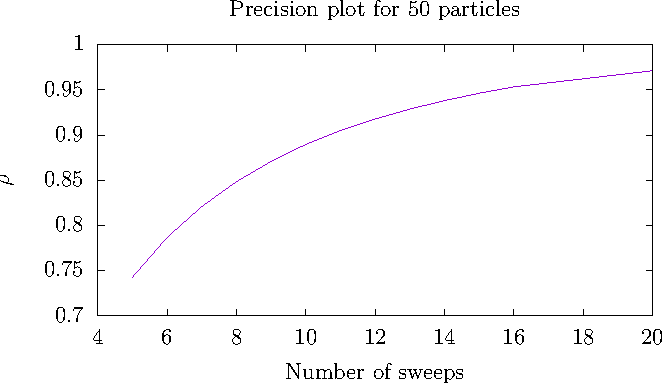
\includegraphics[width=0.9\textwidth]{Figures/condFracSweeps.pdf}
    \caption{\textit{SF condensate fraction as a function of number of sweeps of the DMRG algorithm. A max bond dimension of 250 was used.}}
    \label{fig:sweepdependence}
\end{figure}
Furthermore, one observes numerically, that increasing the maximal bond dimension $D$ results in a more accurate long-range representation of correlations. Thus, calculating correlation functions for various values of $D$ is a great way of estimating the convergence of the correlations for a given length scale [Schollwock].


\subsection{Visualization of density matrices}
One way of displaying the correlations of the system is to plot its density matrix, whose entries are given by
\begin{equation}
	\rho_{i,j} = \bra{\psi} \hat{a}_{i}^{\dag} \hat{a}_j \ket{\psi} \; .
\end{equation}
\begin{figure}[h!]
    \centering
    \begin{subfigure}[t]{0.49\textwidth}
        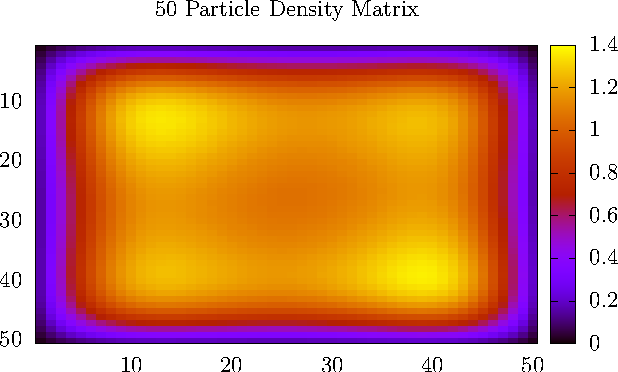
\includegraphics[width=\textwidth]{Figures/DensityMatSF20sweeps.pdf}
        \caption{\textit{Norm value of density matrix entries for $U/J = 0$.}}
        \label{fig:DensityMatSF}
    \end{subfigure}
    ~
    \begin{subfigure}[t]{0.49\textwidth}
        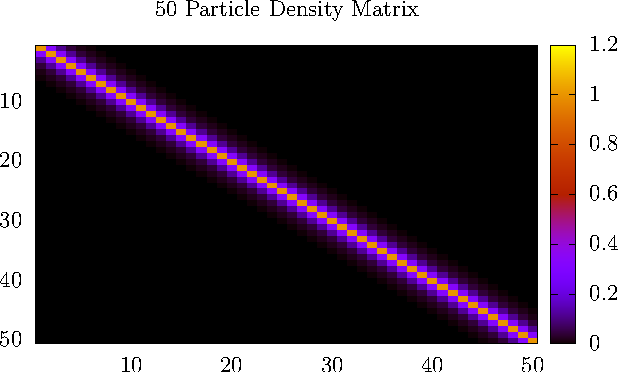
\includegraphics[width=\textwidth]{Figures/DensityMatMI.pdf}
        \caption{\textit{Norm value of density matrix entries for $U/J = 12$.}}
        \label{fig:DensityMatMI}
    \end{subfigure}    
\end{figure}
Figures \ref{fig:DensityMatSF} and \ref{fig:DensityMatMI} show the density matrix of the 50 particle system plotted for the Superfluid and the Mott-Insulator limit respectively. In the SF limit long-range correlations are present, which is seen by large off-diagonal elements. However, as discussed previously, in the MPS approximation all correlations decay exponentially, which causes issues for the elements furthest from the diagonal (top-right and bottom-left corner). This exponential decay is illustrated in figure \ref{fig:expDecayCorrFunc}.
In the MI limit no interaction takes place between sites and the correlation length is zero,  leading to a correlation matrix consisting only of diagonal elements of equal magnitude. Figure \ref{eq:MI_lim} shows some off-diagonal elements of low, but not zero, magnitude, since it is made for $U/J = 12$, meaning the system is not a pure Mott-Insulator.
\begin{figure}[h!]
	\centering
	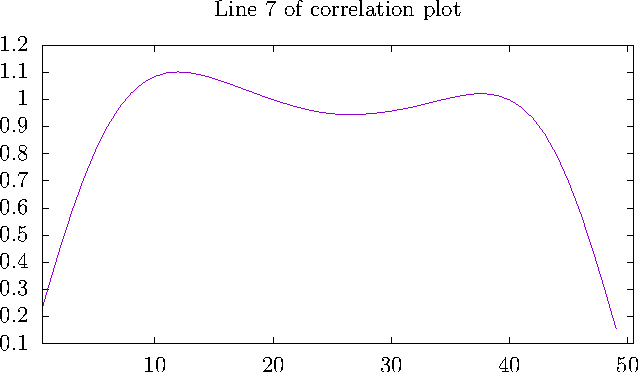
\includegraphics[width=0.9\textwidth]{Figures/row7DensityMatSF.pdf}
	\caption{\textit{Correlation function plotted as a function of distance. The data is from the Superfluid correlation-matrix displayed in figure \ref{fig:DensityMatSF}.}}
	\label{fig:expDecayCorrFunc}
\end{figure}